\chapter{Software methodology} \label{chapter5}

As discussed before in section \ref{Sec:3}, the designers of CNC machines for hobbyists and small scale applications rarely design an integrated software platform i.e. all sequential steps of the software process flow are NOT integrated into a single easy to use platform for the end-user. There could be multiple reasons for doing the same as discussed before. Not having enough knowledge about software development and design could be one of them. The process flow being considerably shorter as compared to what is commonly used in professional and commercial applications could be another. Hence, the sequential steps for the same have been elaborated below.

\section{Schematic design software}

The first and foremost step in PCB design and fabrication is designing a schematic for the same. From the same schematic, an equivalent board file is designed. A schematic merely represents the interconnection between various electronic components and doesn’t give any idea regarding how components are placed or appear on an actual PCB after it has been successfully manufactured and assembled in its entirety. However, the board file (.brd) gives the designer an exact idea regarding the area, footprint and placement of all electronic components in actual sense and also relative to each other. Hence, generating a proper board file is of utmost importance to the designer as this is the first step in our software process flow. \par

In our CNC machine, EAGLE(R) is being used to design the schematic as well as the board file for the schematic design. They appear as separate files and on different tabs/windows on the EAGLE software.  It should be noted that Eagle being a professional PCB design software offers a multitude of features. One of them being able to fabricate multilayered PCBs. Firstly, it should be noted that the designed CNC machine is capable of manufacturing only single-sided PCBs. In the worst-case scenario, the user may opt to manufacture a single layer (top or bottom) out of many possible layers present in the PCB using the concerned CNC machine. Secondly, our CNC machine’s associated software flow doesn’t include an image processing section so the user should be aware that the Gerber files generated by Eagle for a particular board would be generated “as is” and processed further without taking into consideration any possible faults that may occur or that may still remain in the board file. Following is a sample board file shown in the Eagle environment along with its corresponding schematic. \par


\begin{figure}[h]
\begin{center}
\hspace{-45mm}
 \begin{subfigure}{0.5\textwidth}
  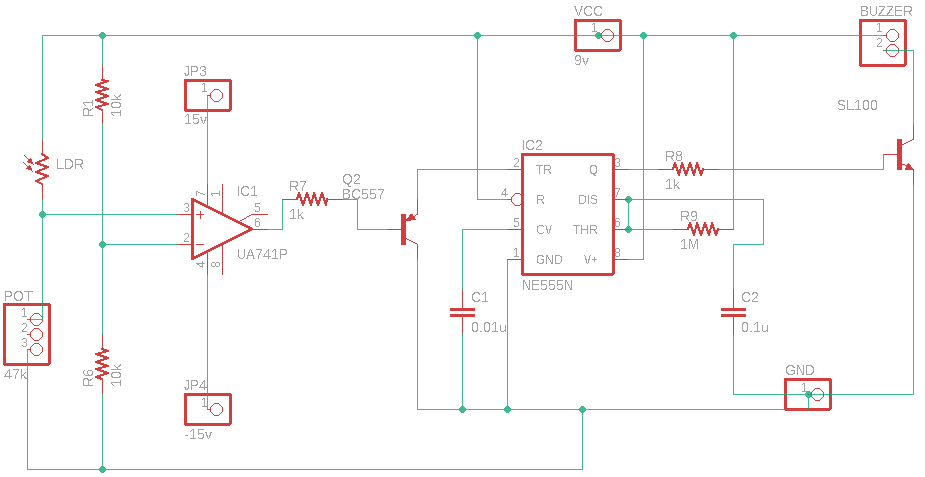
\includegraphics[scale = 0.8]{Chapter_5/sample_schematic.png}
  \caption{Schematic for an Intruder alarm circuit} 
  \label{fig:ckt_sch}
 \end{subfigure} \\
 \end{center}
 \begin{center}
 \begin{subfigure}{0.5\textwidth}
  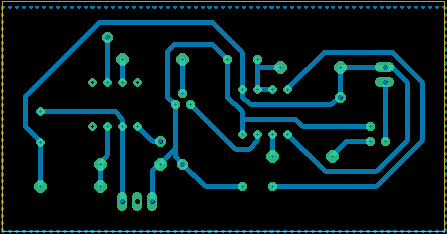
\includegraphics[scale = 1.2]{Chapter_5/sample_board.png}
  \caption{Board file for an Intruder alarm circuit}
  \label{fig:ckt_brd}
 \end{subfigure} 
\end{center}

 \caption{A sample schematic and its corresponding board file used to test the CAM processor wizard in Eagle software}
 \label{fig:sample_ckt}
\end{figure}


After checking for any possible faults in the board file regarding traces, routing, clearances etc. the corresponding Gerber files are generated. To do so, the CAM processor icon (which is available only in the board view) is selected and the appropriate layers are selected for generation of the corresponding Gerber files. Now since the concerned CNC is only capable of manufacturing single-sided PCBs, Gerber file of either the top or bottom layers is only generated. Drill files are also pre-generated which should be ignored since the CNC is capable of only engraving the wire tracks and is not capable of drilling any holes with the drilling equipment available to it. The output file paths for the generation of the Gerber files are usually fixed however, they can be changed wherein required. Once the required Gerber file is generated, it concludes the first step of the software process flow. Following is the image from the procedure. \pagebreak

\begin{figure}[h]
    \centering
    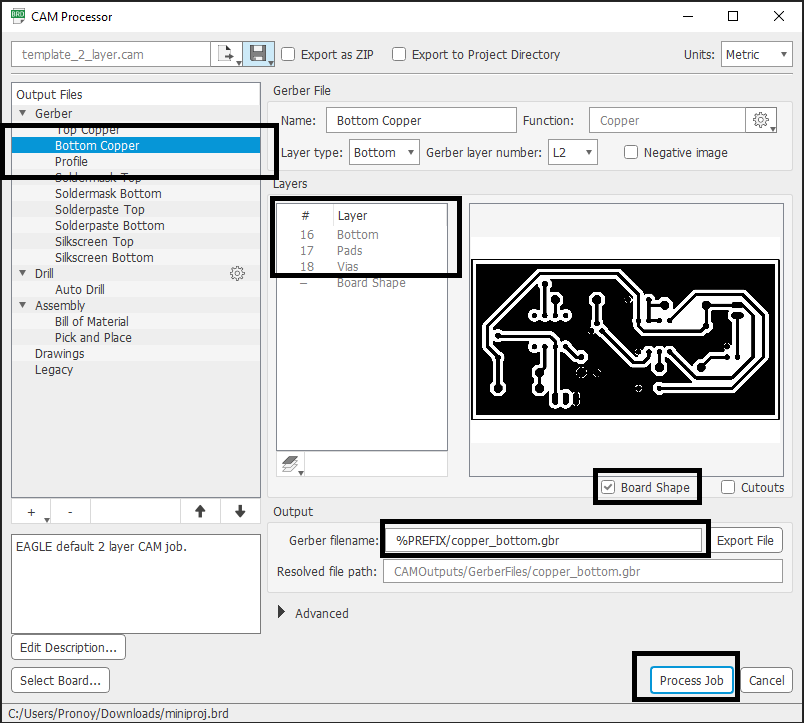
\includegraphics[scale = 0.75]{Chapter_5/cam_processor_dialog.png}
    \caption{A snapshot of the CAM processor dialog box in Eagle (Starting from top left to bottom right): The layer for which the Gerber will be generated, the sub layers included, whether to incorporate the shape of the board, file name and location and \textbf{Process Job} button}
    \label{fig:cam_dialog}
\end{figure}


\section{G code generation} \label{gcodegen}

The next step is to generate the g code corresponding to the Gerber file obtained from the previous step. The software process flow moves online at this stage and hence requires internet access. G-code instruction of a PCB board is generated through the online platform \href{http://copper.carbide3d.com/}{Carbide3D} (\url{http://copper.carbide3d.com/}). It is a free (however, not open-source) software for various CNC jobs and has multiple variants of itself for other specialisations such as woodwork, sheet metal engraving, carving, sculpting etc. \par

As soon as the online application is opened, it asks the user to enter the dimensions of the material in either of the desirable units namely mm and inches and also asks the user the concerned job type (i.e whether the top or bottom of the board is supposed to be traced). Followed by this it asks the user to upload the concerned Gerber file. It should be noted that by virtue of using Eagle software, dedicated Gerber files are obtained for each of the layers i.e. a wrong choice of the job type (top or bottom) won’t affect the final job. The user gets to choose the tool bit that is going to be used as well. \par

\begin{figure}[h]
    \begin{subfigure}{0.5\textwidth}
    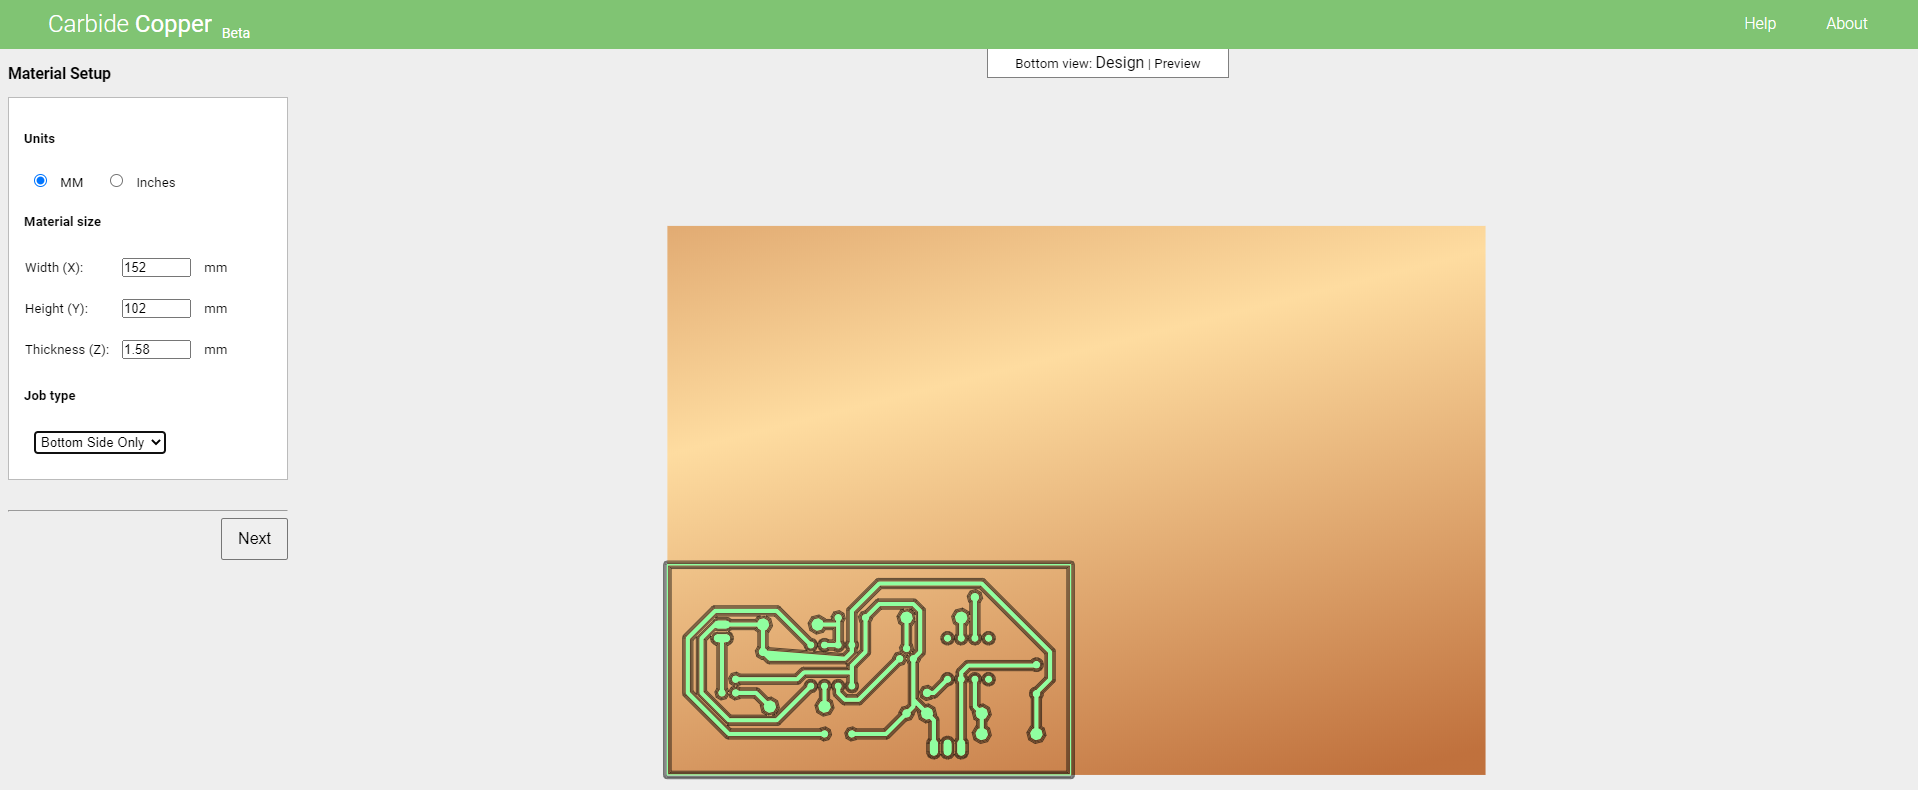
\includegraphics[scale = 0.15]{Chapter_5/g_code_1.png}
    \caption{Choosing the system of units and board dimensions}
    \label{fig:g1}
    \end{subfigure}
    \begin{subfigure}{0.5\textwidth}
    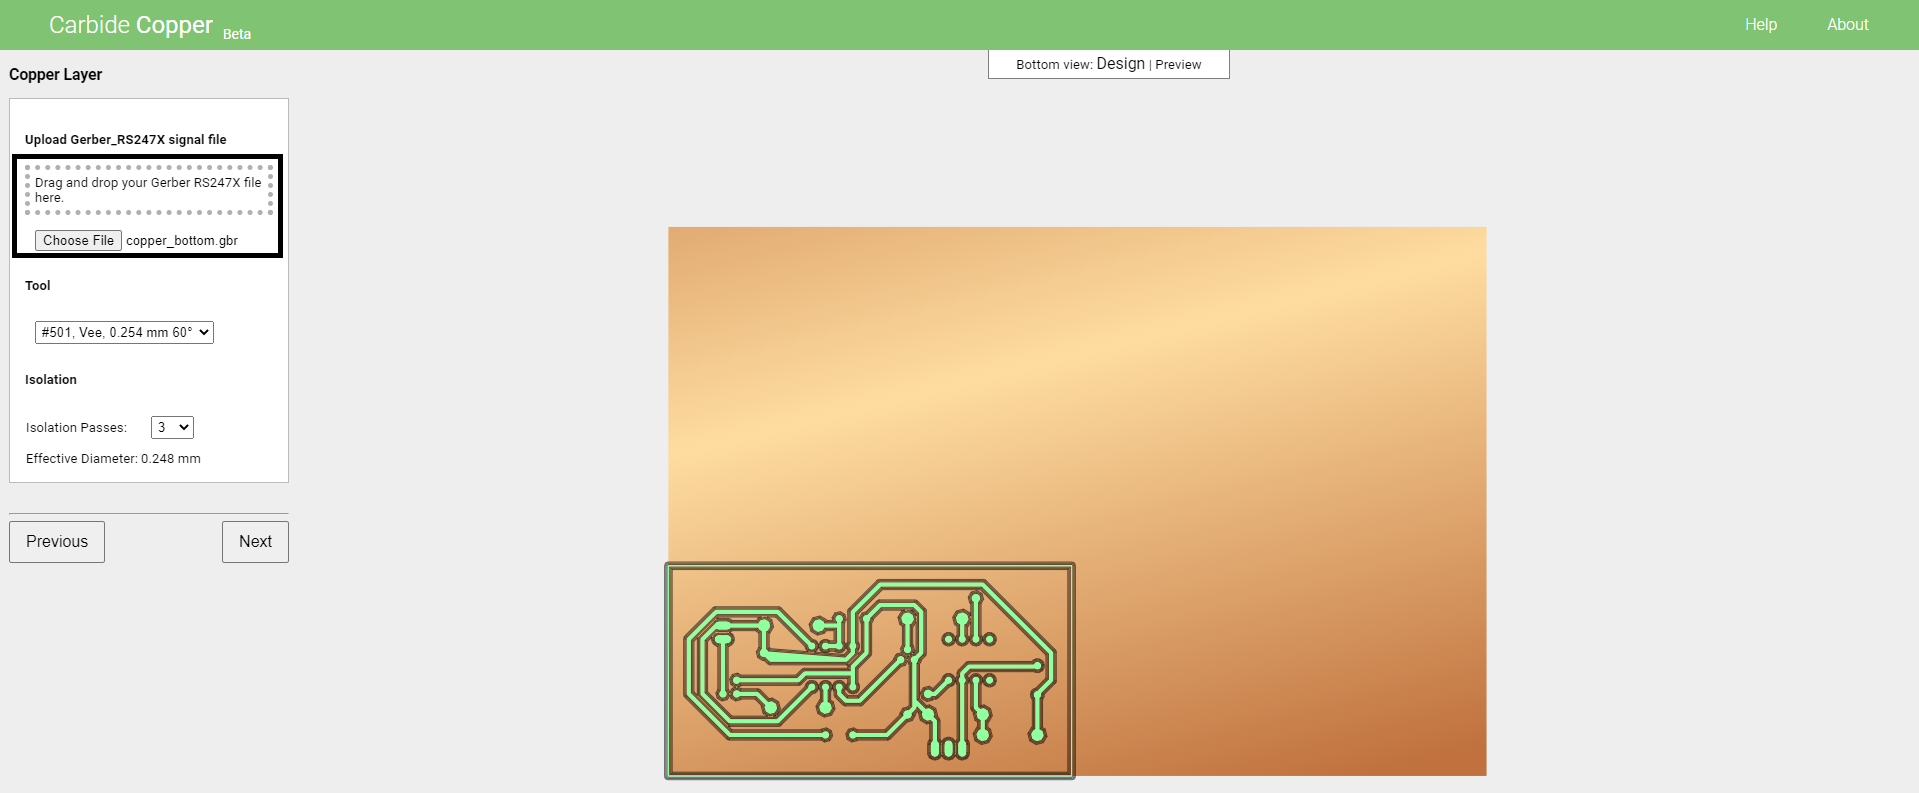
\includegraphics[scale = 0.15]{Chapter_5/g_code_2.png}
    \caption{Uploading Gerber file from the previous step (outlined in black)}
    \label{fig:g2}
    \end{subfigure}
    \caption{The first two steps for G-code generation}
    \label{fig:g12}
\end{figure}

This is followed by asking the specifications regarding the drilling job of the concerned PCB which should be completely ignored. This step is followed by the routing step where again the tool dimensions for engraving purposes will be asked. Designers at this stage can choose to give various dimensional offsets if the need arises or else may choose to skip this step. Also if the boundary cutout for a PCB needs to be made it can be chosen at this stage itself. This step is followed by a relatively minor step of choosing whether to generate an area rub-out or not and any specialized tool to do the same. The following step successfully generates the G-code for the PCB and can be downloaded into the user’s local machine. The software at each stage provides a preview of what is going to be traced out by the final CAM processor. Generating a G-code file for a PCB and saving it to local storage concludes the penultimate step in our software process flow. Following are some snapshots taken from this step of the software process flow. \par

\begin{figure}[h]
    \begin{subfigure}{0.5\textwidth}
    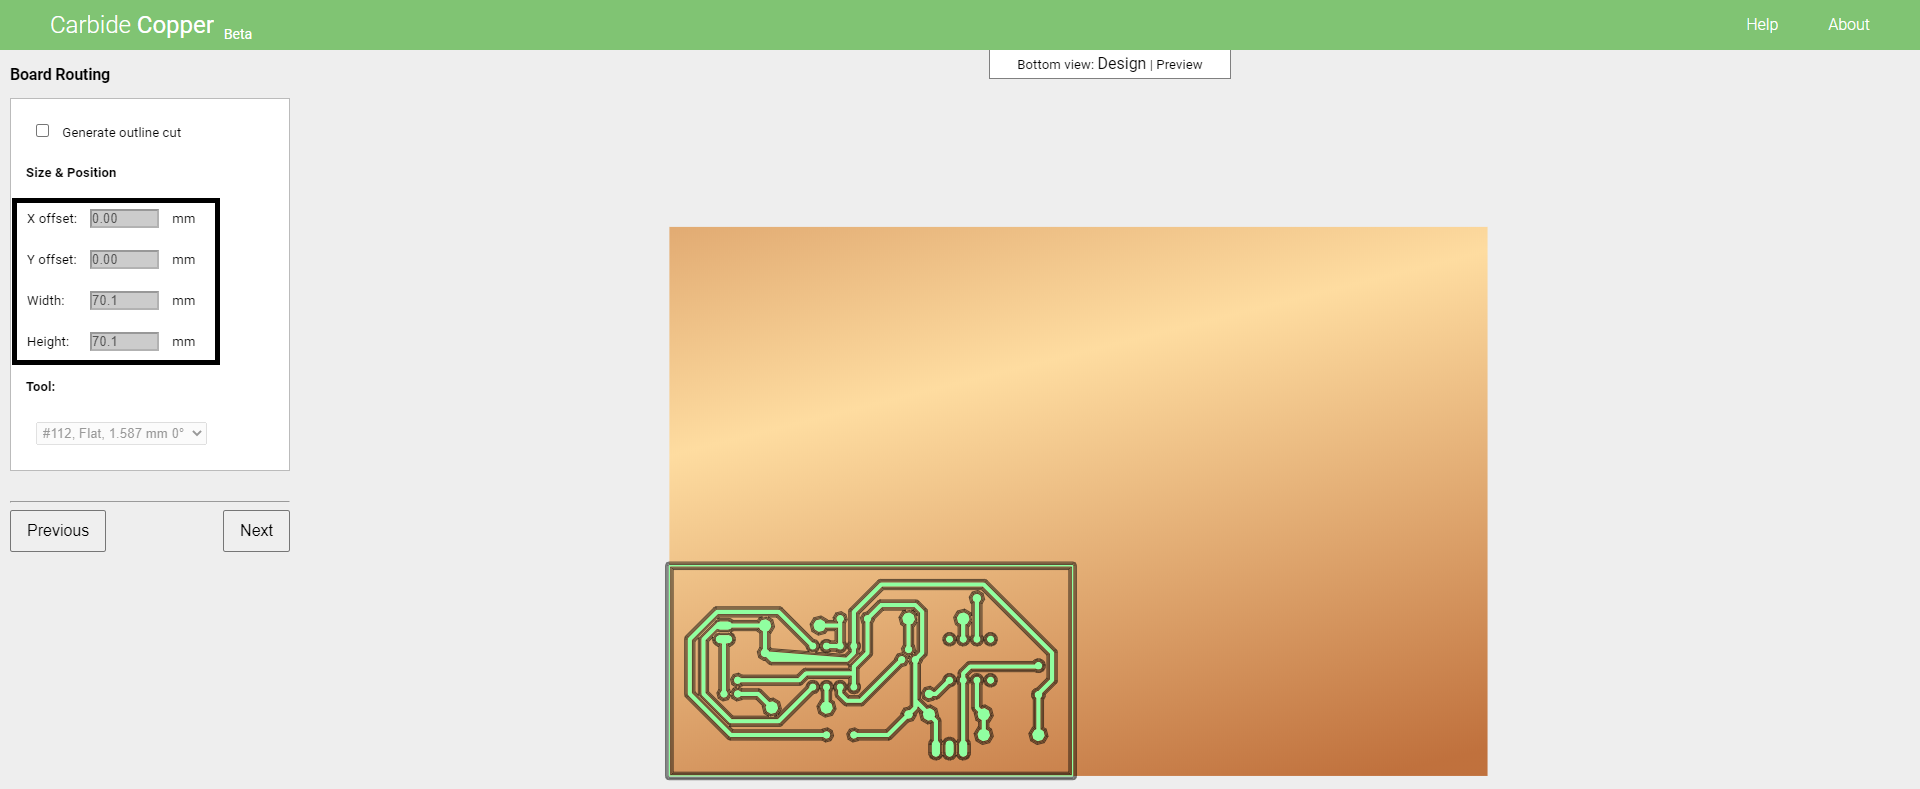
\includegraphics[scale = 0.15]{Chapter_5/g_code_3.png}
    \caption{Routing and offset based settings (outlined in black)}
    \label{fig:g3}
    \end{subfigure}
    \begin{subfigure}{0.5\textwidth}
    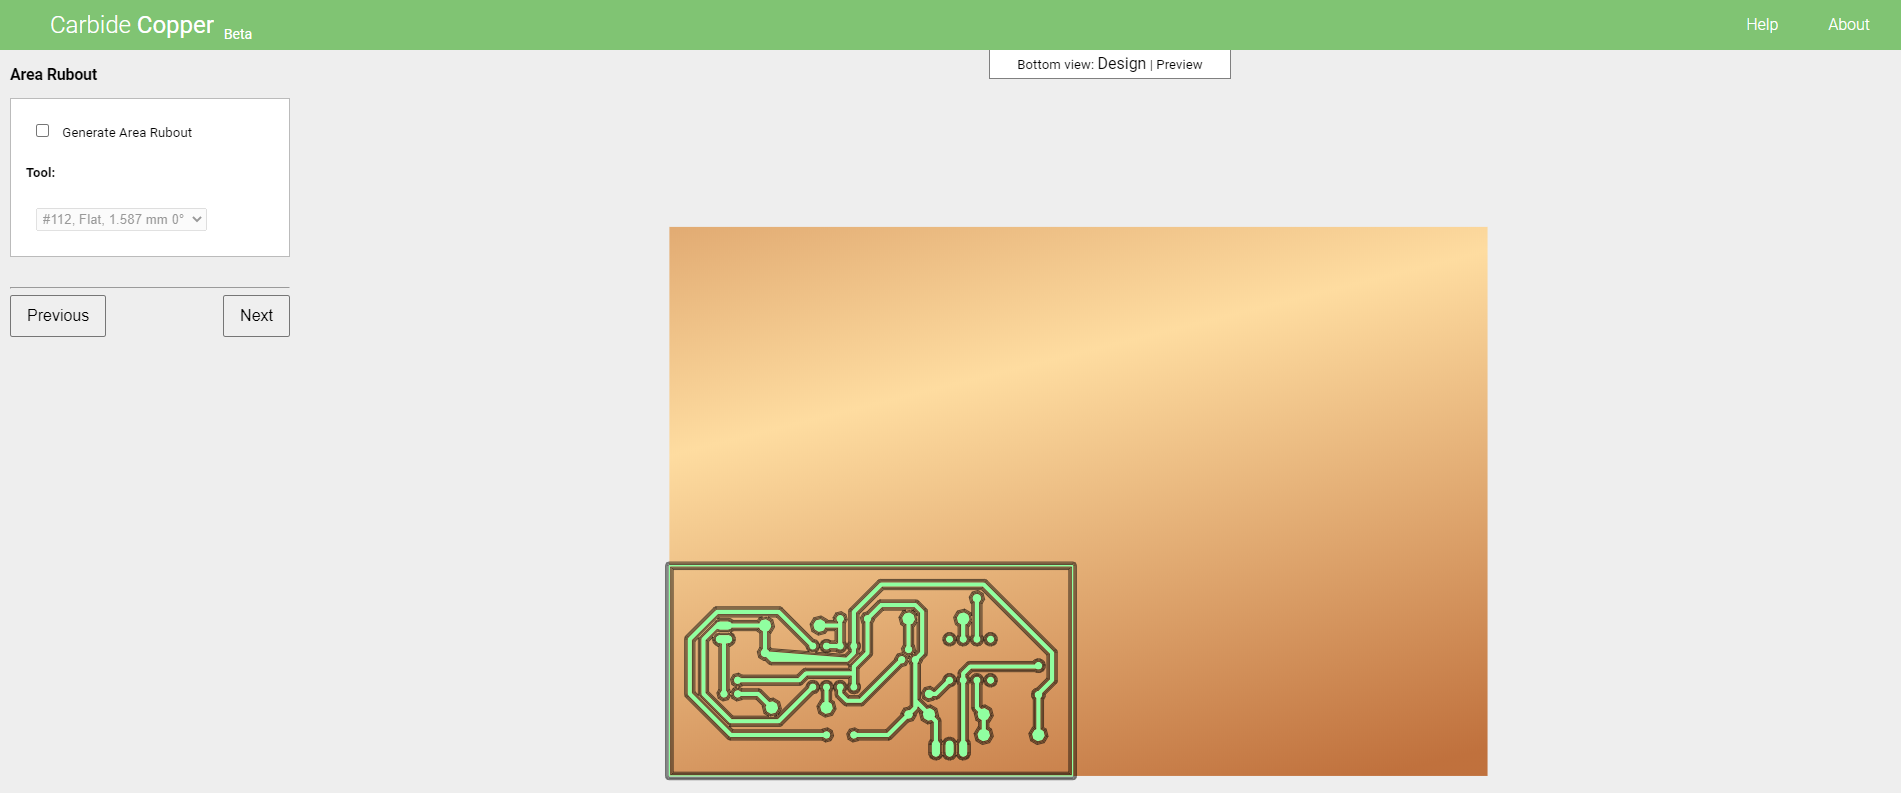
\includegraphics[scale = 0.15]{Chapter_5/g_code_4.png}
    \caption{Options for area rub out and outline cut (outlined in black)}
    \label{fig:g4}
    \end{subfigure}  
    \begin{center}
    \begin{subfigure}{0.5\textwidth}
    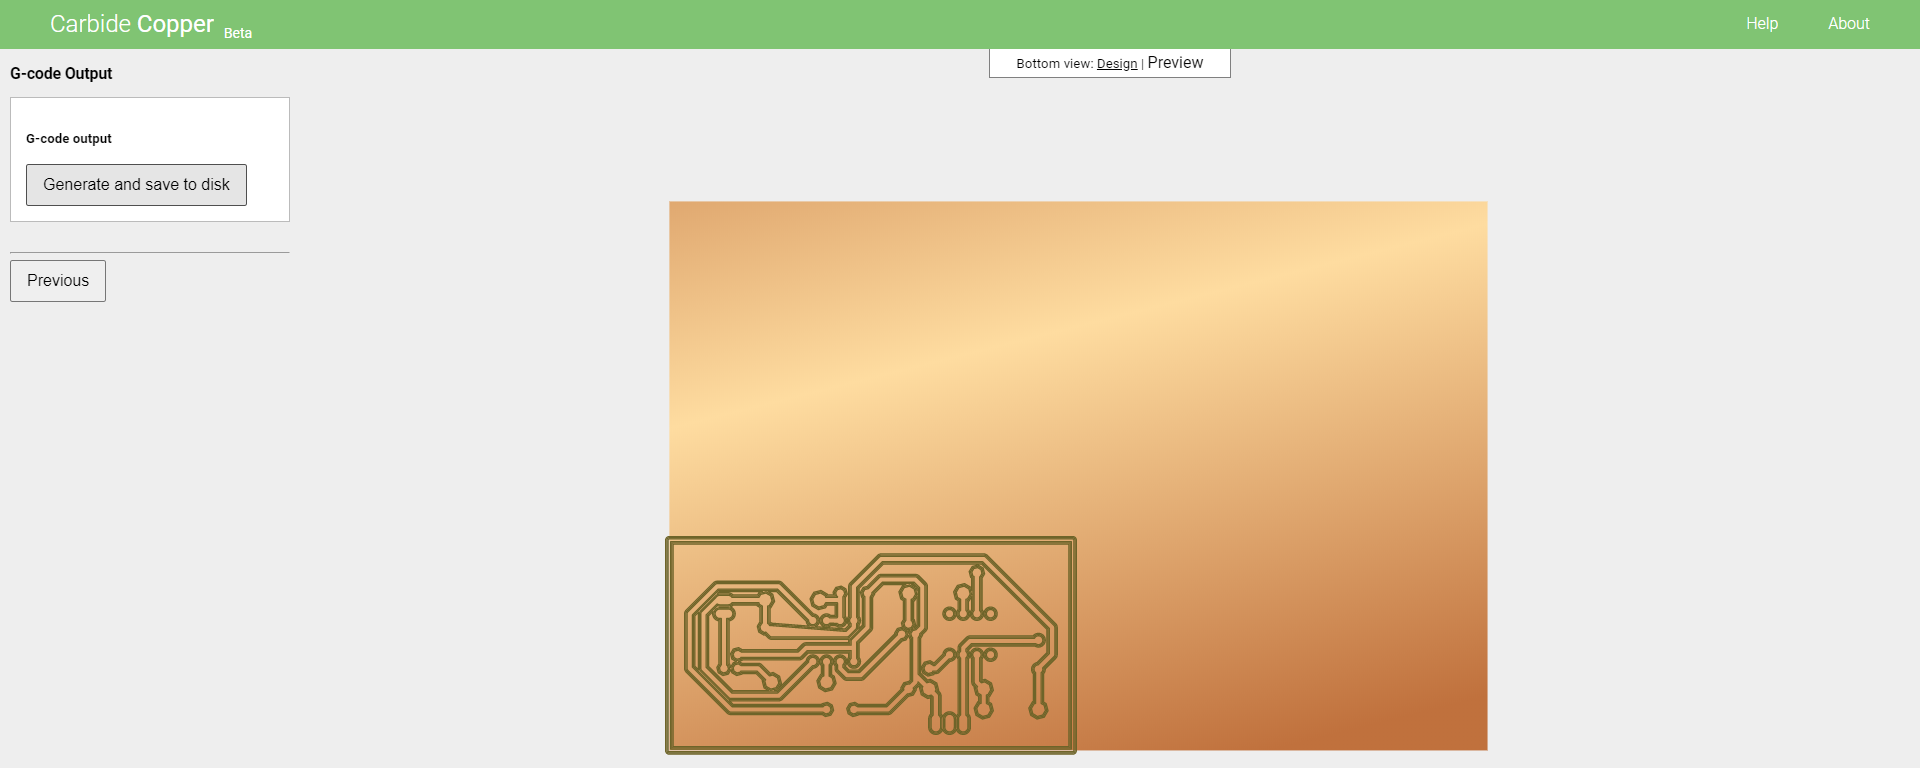
\includegraphics[scale = 0.15]{Chapter_5/g_code_5.png}
    \caption{Downloading the generated G-code file to disk (outlined in black)}
    \label{fig:g5}
    \end{subfigure} 
    \end{center}
    
    \caption{The final steps for G - code generation}
    \label{fig:g345}
\end{figure}

\section{CAM processor}

The final section of the software flow is responsible for sending the obtained g code to the CNC machine which is understandable by the same. To do so the software must be able to recognise the port to which the Arduino board (together with which the CNC shield is connected). There would be two sets of software required for this step i.e. the Arduino compiler (along with the IDE if possible) and the Universal G code sender for the concerned OS platform. \par

To begin with, the Arduino IDE (or whichever relevant text editor is used) is opened up and only a single line of program code is compiled which is given below.

 {\fontfamily{qcr}\selectfont \#include <grbl.h>}

This includes the Gerber header files into your Arduino project i.e it gives a way to convert standard g code instructions to Arduino understandable commands. For e.g. a single movement of the drill head is converted into a series of digital outputs (PWM signals to be precise) on the pins connected to the CNC shield which are then fed into the motor assembly connected with the shield. Since this header file is usually not an inbuilt file or library in the Arduino IDE it needs to be downloaded from external resources such as the official and updated GitHub repository of \href{https://github.com/gnea/grbl}{grbl} - \url{https://github.com/gnea/grbl}. After extracting the zip archive the bin folder contains a readymade .ino file which can be simply opened and uploaded to the board (the file contains only the above line). After successfully doing so the serial monitor is opened. It is worthwhile to note that the serial monitor, in this case, acts as an excellent CLI for directly interacting with the motors via the CNC shield and via the grbl parser. Following are a few simple commands which can be used in this instance of the serial monitor. \par

% ## insert table of simple grbl commands ## %

This concludes the Arduino and grbl setup phase of the CAM processing.

After this basic setup, we can proceed to send the g code files generated in the previous step to the complete CNC assembly. To do so we would be needing a g code sender here, the Universal G code sender will be used (an appropriate version can be downloaded from \url{https://winder.github.io/ugs_website/download/}). Once the software is downloaded and extracted from its archive it is opened. Now, before proceeding onto uploading the obtained G code in the previous step the port and the baud rate should be the same as the one used in the previous phase (port to which the Arduino is connected and the baud rate that was being used for the serial monitor). After this initial setup, the \textbf{connect} icon is pressed (which is located alongside the baud rate selector). If all interfacing has been done properly this will lead to a successful connection between the software and hardware which will be indicated by this icon turning green. If it is not so the user can choose to refresh the ports and the baud rate (this step shall clear any unsent data from each of the COM ports and shall reset the baud rate to a default of 115200). However, it should be noted that the \textit{active} state could still be \textit{ALARM} which can be unlocked by choosing one of the machine actions from Menu bar. \par

% ## insert table of software states ## %

Following this, the G code from the previous step can be directly loaded by choosing your file in the \textit{file input} by clicking on the browse button. However, general testing of the motors is always recommended. This software platform is universal in nature as well as feature-rich so it has a custom jog controller (\textit{jog} in the sense small but finite and user-controlled steps). All the connected motors can be rotated in both the directions by clicking on the $\boldsymbol{+}$ and $\boldsymbol{-}$ icons. A single press of this button corresponds to a single input pulse to the respective motors. Multiple presses may be needed to emulate an actual machine movement. All the implicit G code generated while testing the motors can be seen on the console on the bottom right. After some basic testing, the G code in the previous step is loaded and the CNC job is activated by clicking on the \textbf{RUN} button. If all goes well the CNC machine should begin its job immediately as per the commands written in the G code file. The movements of the tooltip could be visualized in 3D by choosing the 3d visualiser window from the Window option in the menu bar. It should be noted that the Grbl being a fully compiled parser for G code it could throw errors at the beginning itself on encountering unsupported commands. These commands could either be unsupported by the current version of the software OR could be machine codes (M codes) which are beyond the capabilities of the CNC machine. To find out or detect such commands the parser simply \textit{reads all the ports} and finds out unavailable port addresses or ports which are not interfaced to any peripheral. After successfully removing all the errors depending on the complexity of the G code the CNC job would run successfully and produce the final engraved/etched PCB design. This concludes the overall software process flow and satisfies the main objective of this project.


\section{Overall software process flow}


\begin{figure}[h]
 \centering
 \tikz [every node/.style = draw]
 \graph { foo -> bar -> blub };
 \caption{Overall software process flow represented as a simple flowchart}
 \label{fig:soft_process_flow}
\end{figure}

% Draw overall software process flow %

\hspace{-13.7mm}
\textbf{Step 1}: Designing the schematic and the board file in Eagle or any other suitable schematic design software and then exporting the Gerber files from the same. \\[5mm]
\textbf{Step 2}: Generating G-code corresponding to the Gerber files in \href{http://copper.carbide3d.com/}{Carbide3D} (\url{http://copper.carbide3d.com/}) (section \ref{gcodegen}) and downloading the same to the local machine. \\[5mm]
\textbf{Step 3}: Importing generated G-code file from the system into Universal G-code sender software for execution. \\[5mm]
\textbf{Step 4}: Including the Grbl header file in an Arduino file (.ino) and compiling and uploading the same to the Arduino UNO board. \\[5mm]
\textbf{Step 5}: Executing the G-code file from Universal G-code sender to instruct the CNC machine to process the job.
